%% https://eurompi.github.io/cfposter.html
%%
%% Submission Deadline: July 25, 2020 (AOE)
%% 
%% Notification of Acceptance: August 15, 2020
%% 
%% Submission Instruction:
%% 
%% All poster submissions must include:
%% 
%% A short abstract (175 word maximum).
%% An extended abstract (3 pages maximum, including figures and
%% references, and formatted according to the "sigconf" style in the ACM
%% 2017 Template (http://www.acm.org/publications/proceedings-template)).  
%% A poster draft. Note that complete results are not necessary. It is
%% acceptable to have placeholders for last-minute results. 
%% Poster format should be A0 page size (either portrait or
%% landscape). See the attached size guide instructions for more
%% details. 
%% The abstracts and posters will NOT be published in the conference
%% proceedings by ACM-ICPS. In case of acceptance, posters will be
%% presented at the conference and, if the authors agree, they will be
%% published on the EuroMPI/USA'20 poster web page.

\documentclass[sigconf,nonacm]{acmart}
\usepackage{graphicx}
\usepackage{url}
\usepackage{todonotes}

\def\Underline{\setbox0\hbox\bgroup\let\\\endUnderline}
\def\endUnderline{\vphantom{y}\egroup\smash{\underline{\box0}}\\}
\def\|{\verb|}
%
\long\def\comment#1{}
%

\begin{document}

\title{A Report of MPI International Survey}

\author{Atsushi Hori}
%\email{ahori@riken.jp}
\author{Takashi Ogura}
%\email{t-ogura@riken.jp}
\author{Balazs Gerofi}
%\email{bgerofi@riken.jp}
\author{Jie Yin}
%\email{jie.yin@riken.jp}
\author{Yutaka Ishikawa}
%\email{yutaka.ishikawa@riken.jp}
\affiliation{\institution{Riken CCS}}

\author{George Bosilca}
%\email{bosilca@icl.utk.edu}
\affiliation{\institution{The University of Tennessee}}

\author{Emmanuel Jeannot}
%\email{emmanuel.jeannot@inria.fr}
\affiliation{\institution{Inria}}

\maketitle

\section{Abstract}

The Message Passing Interface (MPI) plays a critical part in the
parallel computing ecosystem, a driving force behind many of the
high-performance computing (HPC) successes. To maintain its relevance
to the user community---and in particular to the growing HPC community
at large---the MPI standard needs to identify and understand the MPI
users' expectations and concerns, and adapt accordingly.

%
Existing studies on MPI uses are focused on a restricted target domain,
such as the Exascale Computing Project (ECP)~\cite{ECP} study
conducted in 2017~\cite{osti_1462877} that focused 
on MPI usage in the context of ECP applications; and/or those that are
geographically 
constrained to a single laboratory, funding agency or at best, country.
%In 2017, ECP~\cite{ECP} conducted a survey for MPI users in the ECP
%project to reveal how MPI would/should be integrated with ECP
%applications~\cite{osti_1462877}.
%
Such studies inspired us to conduct a larger study, not focused on
high-end HPC, but targeting a wider audience and involving a larger
spectrum of geographically distinct users. Since MPI has been a widely
used vehicle for high-performance computing for decades, this
larger-scale questionnaire survey would be beneficial not only for
deciding the future direction of MPI, but also for understanding the
feature differences of MPI users among countries and/or regions of the
world.
% Our survey is international and targets novice to expert
% users, hoping to be a complement to the ECP survey.

This survey was conducted from February to June 2019, and at the time of
this writing has gathered more than 800 answers from 42 countries.
%
This report, based the July 2020 results of the survey,
focuses on the MPI users communities awareness of MPI features.
% which MPI features MPI users know and which ones they do not.
%
This survey reveals the staggering fact that most MPI users make use
of a small subset of the MPI API, a subset that mostly avoids features
introduced after MPI 2.2, released in 2009, such as PMPI, dynamic
process creation, and persistent communications. Further, the survey
reveals that many MPI users learn MPI from the internet and/or some
form of online documents, highlighting a shift in the education of the
target community.
%
These two outcomes seem to suggest that many MPI users failed to receive the
information about new MPI features because most internet sources are outdated
and lack support for them. It also suggests that one quick way to address this
is to provide the necessary education, possibly as part of the MPI Forum effort.

\section{Survey}

\begin{table}[htb]%
%\footnotesize
\scriptsize
\begin{center}%
\begin{tabular}[t]{cc}

\begin{minipage}[t]{0.5\hsize}
\begin{center}%
\caption{\small Top 10 Countries of Participants}
\label{tab:countries}%
\begin{tabular}{c|l|c|c}%
\hline%
Rank & Country & \# Ans & Percent \\%
\hline%
1 & Germany 	& 159 & 18.68 \\%
2 & France 	& 125 & 14.69 \\%
3 & Russia 	& 94  & 11.05 \\%
4 & UK 		& 67  &  7.87 \\%
5 & Japan 	& 64  &  7.52 \\%
6 & USA 	& 58  &  6.82 \\%
7 & Italy 	& 57  &  6.60 \\%
\hline
8 & Switzerland & 40  &  5.76 \\%
9 & South Korea & 27  &  3.17 \\%
10 & Austria 	& 26  &  3.06 \\%
\hline%
\end{tabular}%
\end{center}%
\end{minipage}

\hspace{1mm}

\begin{minipage}[t]{0.5\hsize}
\begin{center}%
\caption{\small Top500 Performance System Share (June 2020)\cite{Top500}}
\label{tab:top500-share}%
\begin{tabular}{c|l|c}%
\hline%
Rank & Country & Perf. Share [\%] \\%
\hline%
1  & USA 	  & 28.18 \\%
2  & China 	  & 25.64 \\%
3  & Japan 	  & 23.92 \\%
4  & Italy	  & 3.95  \\%
5  & France	  & 3.62  \\%
6  & Germany 	  & 3.11  \\%
7  & UK		  & 1.40  \\%
8  & Canada	  & 1.27  \\%
9  & Netherlands  & 1.12  \\%
10  & Switzerland  & 1.05  \\%
\hline%
\end{tabular}%
\end{center}%
\end{minipage}%

\end{tabular}%
\end{center}%
42 countries, 851 participants\\%
\end{table}%

The points we kept in mind while designing the survey's questions
were: (a) minimizing the number of questions, (b) making them easy to
answer, and (c) avoiding ambiguity. The questionnaire is implemented
by using firstly Google Forms and later Microsoft Forms, and
distributed via emails to major mailing lists such as {\tt
  hpc-announce} and by personal contact to diverse academic and
governmental institutions and vendors. All data, a Python program to
analyze the answers, and all reports published so far (including this
one) are available on
GITHUB.\footnote{\url{https://github.com/bosilca/MPIsurvey.git}}

Table~\ref{tab:countries} shows the number of answers from top-10 countries. It
should be noted that the survey does not ask participants nationality, but
instead ask the most recent (last 5 years) country of employment.

Table~\ref{tab:top500-share} shows the top-10 aggregated system
performance per country as of June 2020. Comparing with
Table~\ref{tab:countries} highlights a big disparity, possibly related
to the number of users or to their dedication of answering an online
survey. In particular it can be noted that only 18 participants from
Chinese institutions answered. We noticed this immediately after
publishing the survey and we have been trying to narrow the gap, but
our efforts were unfortunately not able to change the trend. Overall,
if aggregating the answers geographically, we currently have 65\% of
answers from Europe, 15\% from Asia, 11\% from Russia, and 7\% from
North America.

The countries having more than 50 participants (above the line in
Table~\ref{tab:countries}) are the target of cross-tab analysis. One
may argue that the number of 50 is too small to conduct cross-tab
analysis, however, this threshold was decided to have enough number of 
major countries.

Most answers, around 85\%, come from research organizations
(universities and governmental research institutes).  We think this
diversity reflects not the characteristics of the countries, but
came from the biased questionnaire distribution.

Since the above profiles may bias the analysis of the results,
readers must keep this in mind when considering the background. 

\section{Survey Results}

\begin{table*}[htb]%
%\footnotesize
\scriptsize
\begin{center}%
\begin{tabular}[t]{cc}

\begin{minipage}{0.45\hsize}
\begin{center}
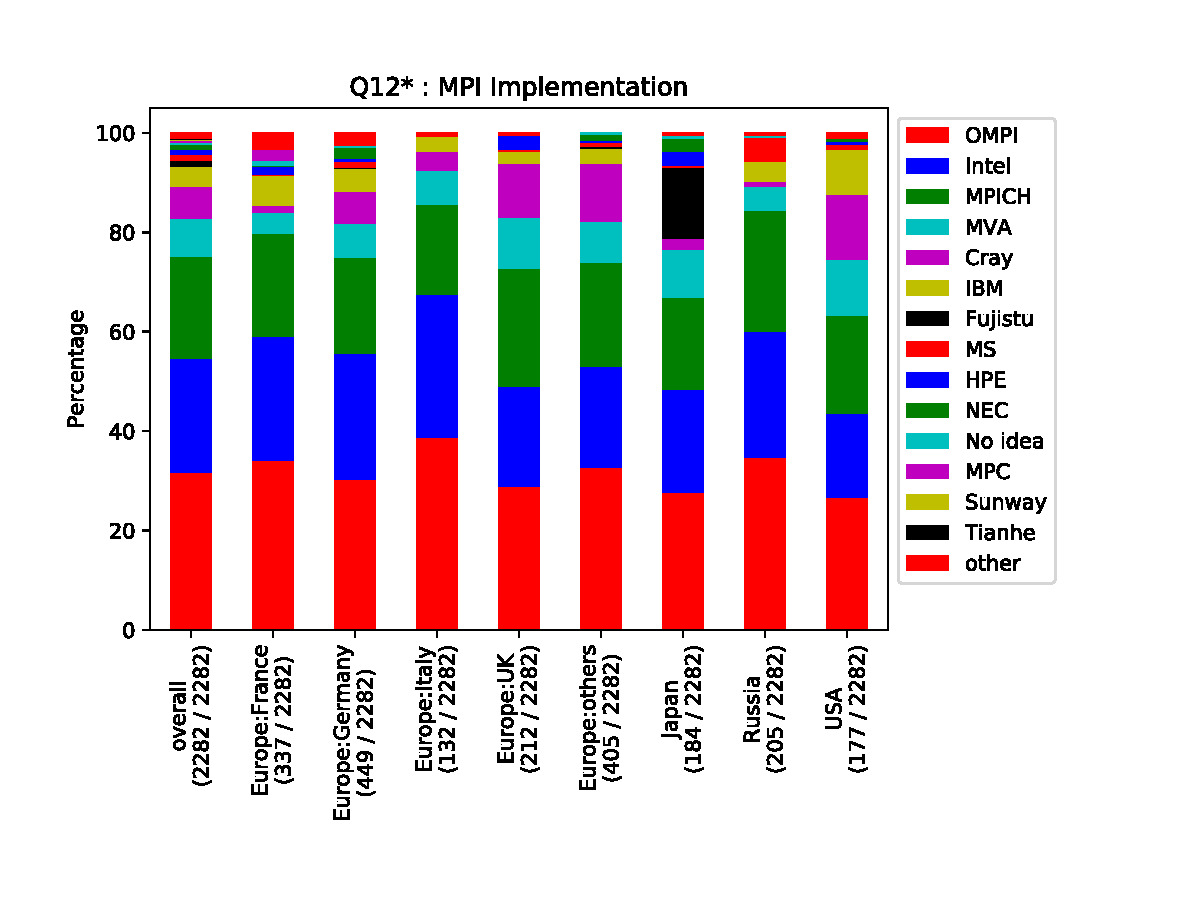
\includegraphics[width=0.9\hsize]{figs/Q12-S.pdf}
\caption{Which MPI implementations do you use?}%
\label{fig:Q12}
\end{center}
\end{minipage}

\begin{minipage}{0.48\hsize}
\begin{center}
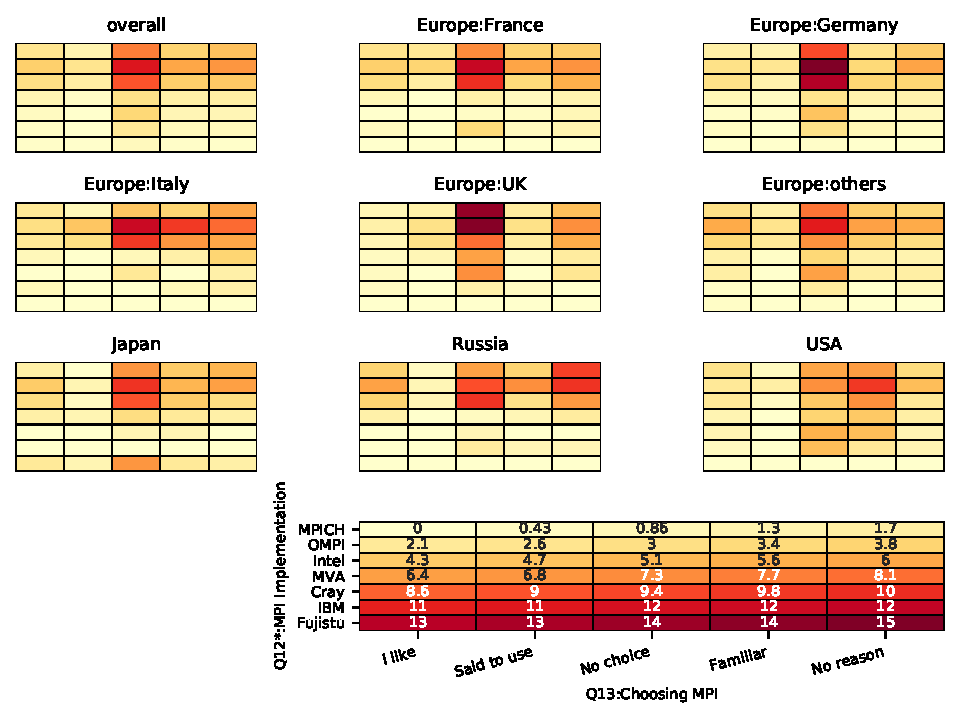
\includegraphics[width=0.8\hsize]{figs/Q12-Q13.pdf}
\caption{Cross-tab: MPI Implementations and choice reason}%
\label{fig:Q12-Q13}
\end{center}
\end{minipage}

\end{tabular}
\end{center}
\end{table*}

\subsection{Choice of MPI Implementation}

Figure~\ref{fig:Q12} shows the result of multiple answer question
asking ``Which MPI implementations do you use?'' Note that the order
in the legend and the orders of bars are reversed. 
With respect to the geographical distribution of MPI implementations,
several patterns stand out. In all countries and regions, Open~MPI
(denoted as 'OMPI'),
Intel~MPI ('Intel') and MPICH dominate more than 60\%. Intel~MPI is
the most 
widely used vendor provided MPI implementation all over the
world. Cray~MPI ('Cray') dominates around 10\% in most countries and
regions. From the less dominant vendors, Fujitsu~MPI ('Fujitsu')
enjoys wider usage than Cray~MPI in Japan, while IBM has visible
presence in both Europe and the US. 
On the other end of the spectrum are research oriented
implementations, such as MadMPI with only a few mentions in
France and ParaStation MPI used exclusively in
Germany (they are not shown in the figure). Italy and Russia mostly
use open source MPI implementations.

Figure~\ref{fig:Q12-Q13} shows heatmaps of cross-tab analysis of the
answers asking ``which MPI implementations do you use?''
(Figure~\ref{fig:Q12} and ``why did you choose the MPI
implementation(s)?'' Legend is located at the lower right
corner. The numbers in the legend cells represent the
percentage and darker color means higher percentage. USA has the most
distributed MPI choices and more US users choose MPI implementations
on their preferences than the other countries.
  
\subsection{Threading Support}

\begin{figure}[htb]
\begin{center}
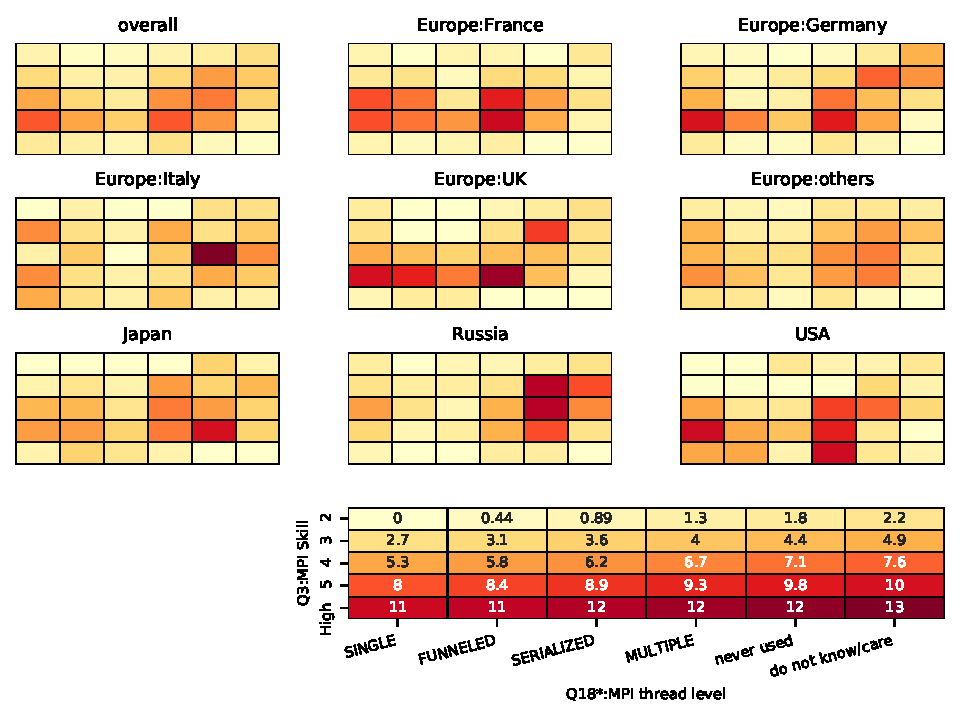
\includegraphics[width=0.8\hsize]{figs/Q3-Q18.pdf}
\caption{Cross-tab: MPI Skill and Thread Level}%
\label{fig:Q3-Q18}
\end{center}
\end{figure}

Figure~\ref{fig:Q3-Q18} shows another heatmap of two questions; ``Rate
your MPI programming skill'' (X axis) and ``Which MPI thread support
are you using?'' (Y axis).
%
France, Germany and UK show a very similar and expected outcome, the
highest users programming skills the more they were tending to use a
more complex programming approach, where threading is an integral part
of the software stack.
% most users declared 5 (higher the number, higher the skill) specify
% MPI thread levels and the most novice users have never used the
% threading support.
The US users exhibit a very differently behavior. Most users seem to
favor the two extremes of the MPI threading support, either {\tt
  MPI\_THREAD\_MULTIPLE} or {MPI\_THERAD\_SINGLE}, irrelevant of their
programming skills.
%
\todo[inline]{The difference here might be due not directly to MPI as
a programming paradigm but to the libraries these users are running
and to their approach to HPC in general. We can't really say this but
having worked on both sides, I realize that in Europe the tendency is
toward small, focused projects, with a clear life expectancy and
little change for a perenial existence. This is the exactly opposite to
US, where the major efforts are going toward software re-usability.}
%
Most interestingly Japan exhibits a very
curious result. Most Japanese users declared high MPI programming skills (5),
however, most of them do not use MPI threading support. This Japanese
anomaly is discussed in~\cite{swopp2019}.

\subsection{MPI Functions}

Table~\ref{tab:Q10-ans}, \ref{tab:Q14-ans}, \ref{tab:Q16-ans}, and
\ref{tab:Q17-ans} show the answer distribution for 4 questions out of
30. Note that the numbers in these tables reflect that these questions
allow participants to choose multiple answers. 
The actual number of participants who answered
each question is noted after the slash (/) of the total number
at the end of each table.

\begin{table*}[htb]%
%\footnotesize
\scriptsize
\begin{center}%
\begin{tabular}[t]{cccc}

\begin{minipage}[t]{0.24\hsize}
\begin{center}%
\caption{\small How did you learn MPI?}%
\label{tab:Q10-ans}%
\begin{tabular}[t]{l|r}%
\hline%
Multiple Choice & \# Answers \\%
\hline%
Articles found on Internet & 439 (51.8\%) \\%
Other lectures or tutorials & 438 (51.7\%) \\%
MPI standard docs & 329 (38.8\%) \\%
Lecture(s) at school & 294 (34.7\%) \\%
Book(s) & 283 (33.4\%) \\%
Never learned MPI & 26 (3.1\%) \\%
other & 51 (6.0\%) \\%
\hline%
\multicolumn{1}{c}{total} & 1860 / 847 \\%
\hline%
\end{tabular}%
\end{center}%
\end{minipage}%

\hspace{1mm}
\begin{minipage}[t]{0.24\hsize}
\begin{center}%
\caption{\footnotesize How do you check MPI specifications when you are writing MPI programs?}%
\label{tab:Q14-ans}%
\begin{tabular}[t]{l|r}%
\hline%
Multiple Choice & \# Answers \\%
\hline%
Online docs. & 579 (68.8\%) \\%
Internet & 566 (67.2\%) \\%
MPI standard docs. & 430 (51.1\%) \\%
I ask colleagues & 188 (22.3\%) \\%
I read book(s) & 108 (12.8\%) \\%
I know all MPI routines & 46 (5.5\%) \\%
other & 11 (1.3\%) \\%
\hline%
\multicolumn{1}{c}{total} & 1928 / 842 \\%
\hline%
\end{tabular}%
\end{center}%
\end{minipage}%

\hspace{1mm}
\begin{minipage}[t]{0.24\hsize}
\begin{center}
\caption{\small Which MPI features have you never heard of?}%
\label{tab:Q16-ans}%
\begin{tabular}[t]{l|r}%
\hline%
Multiple Choice & \# Answers \\%
\hline%
PMPI interface & 465 (66.1\%) \\%
Persistent comm. & 433 (61.5\%) \\%
Dynamic process creation & 383 (54.4\%) \\%
One-sided comm. & 131 (18.6\%) \\%
Communicator operations & 123 (17.5\%) \\%
Point-to-point comm. & 91 (12.9\%) \\%
MPI datatypes & 90 (12.8\%) \\%
Collective comm. & 86 (12.2\%) \\%
MPI w/ OpenMP & 86 (12.2\%) \\%
\hline%
\multicolumn{1}{c}{total} & 1,888 / 704 \\%
\hline%
\end{tabular}%
\end{center}%
\end{minipage}

\hspace{1mm}
\begin{minipage}[t]{0.24\hsize}
\begin{center}
\caption{\footnotesize What aspects of the MPI standard do you use in your program in its current form?}%
\label{tab:Q17-ans}%
\begin{tabular}[t]{l|r}%
\hline%
Multiple Choice & \# Answers \\%
\hline%
Collective comm. & 740 (89.0\%) \\%
Point-to-point comm. & 710 (85.4\%) \\%
MPI datatypes & 521 (62.7\%) \\%
w/ OpenMP (multithread) & 478 (57.5\%) \\%
Communicator operations & 412 (49.6\%) \\%
One-sided comm. & 226 (27.2\%) \\%
PMPI interface & 67 (8.1\%) \\%
Persistent comm. & 61 (7.3\%) \\%
Dynamic process creation & 51 (6.1\%) \\%
other & 20 (2.4\%) \\%
\hline%
\multicolumn{1}{c}{total} & 3,240 / 831 \\%
\hline%
\end{tabular}%
\end{center}
\end{minipage}

\end{tabular}%
\end{center}%
\end{table*}%

Table~\ref{tab:Q10-ans} shows the result of the question asking ``How
did you learn MPI.'' It is a bit surprising that 40\% (323/825) of
participants refer to the MPI standard, despite it's lack of examples
to walk-through. According to the original
data (omitted due to the space limit), one quarter of participants
learned MPI via the internet and/or online documents.

The result of the question asking ``How do you check MPI
specifications when writing MPI programs'' is shown in
Table~\ref{tab:Q14-ans}. More than half of participants refer to the
MPI standard. It is very natural for MPI users to check MPI
specification by referring the MPI standard more often than reading it
for learning. Most notably, the percentage of participants reading
online documents and/or referring the internet occupies 46\% (original
data).

Referring Table~\ref{tab:Q16-ans} and \ref{tab:Q17-ans}, the MPI
features can be categorized into two groups: well-known ones (P2P,
Collectives, and so on) and little-known ones (PMPI, Persistent and
Dynamic process). Surprisingly, this tendency is almost independent
from countries/regions of the participants.

\begin{figure}[bht]
\begin{center}
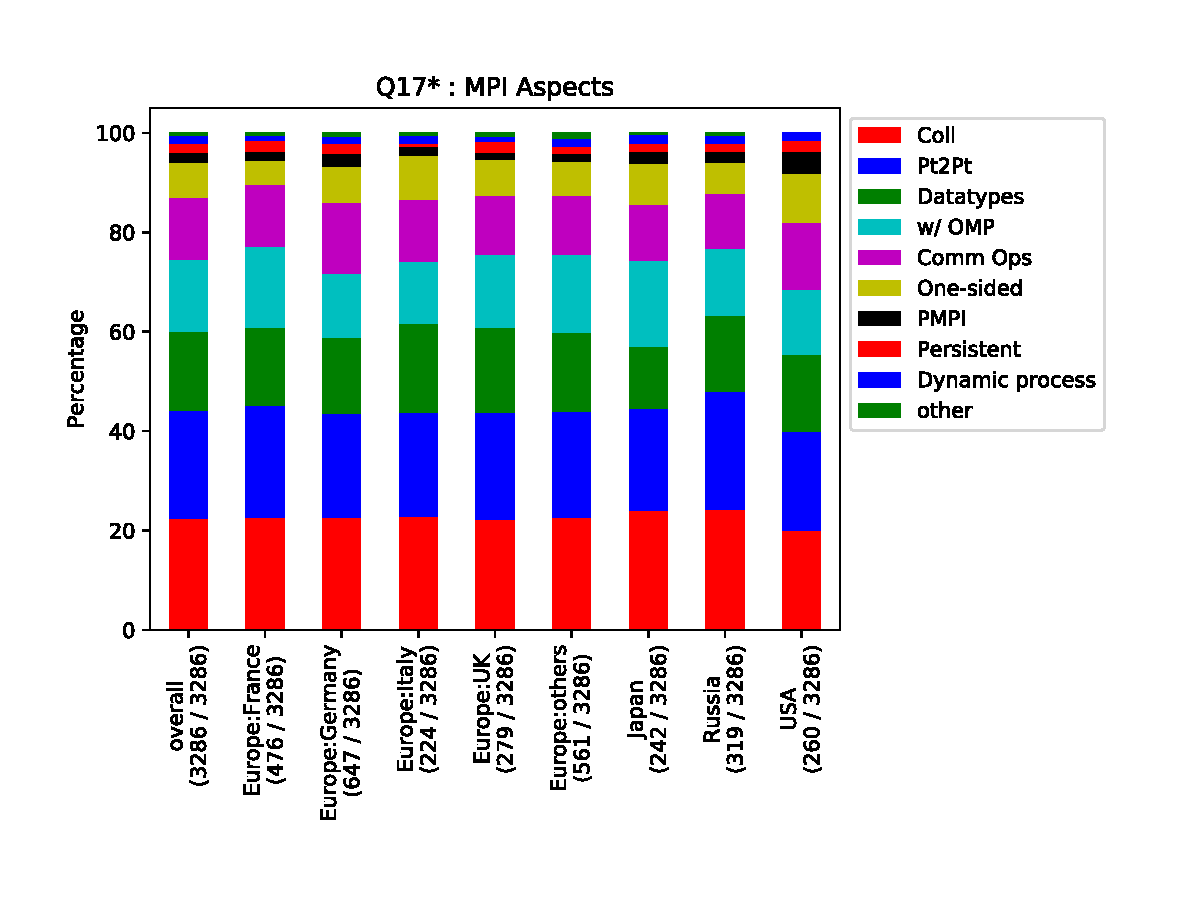
\includegraphics[width=0.8\hsize]{figs/Q17-S.pdf}
\caption{What aspects of the MPI standard do you use in your program in its current form?}%
\label{fig:Q17}
\end{center}
\end{figure}

Among the little-known MPI features, the persistent communication is
one of the important directions being discussed on the MPI Forum\cite{mpi-forum}.
The persistent communication can give implementors room for
optimizing not only P2P but also collective communication
performance.
All those little-known MPI features already appeared in MPI 2.2
released in 2009. Despite the 10-year appearance, those features
fail to be widely accepted.  Why?

One possible answer to this question may come from the survey results
asking participants ``how did you learn MPI''
(Table~\ref{tab:Q10-ans}) and ``how do you check
MPI specifications when you are writing MPI programs''
(Table~\ref{tab:Q14-ans}).
Here a significant number of participants refer to the internet
and/or online documents. These are handy and allow users to get
required information on the fly. However,
these online medias can only be retrieved by
search. To search something, a clue or some keywords must be given.
Say someone wants to search something he/she does not know; how can he/she
find the appropriate key words to obtain the right information?
This could be the responsibility of the information providers. For example,
there is no {\tt See Also} link from the man page of {\tt MPI\_Irecv}
to the corresponding persistent routines in many MPI implementations.

\comment{
Contrastingly, traditional medias such as books, lectures, and tutorials can be
systematic and complete, but not handy.  Once you learned MPI via some
of those traditional medias, you may think that you already know
MPI. Unfortunately, the MPI standard is being updated by MPI Forum. It is
very hard to keep your MPI knowledge up-to-date, especially if MPI is not
your major concern.

The other point we noticed is that many people who chose the ``other''
answer to the question asking ``how did you learn MPI'' said
``reading existing code,'' ``learn by doing,'' ``reverse
engineering''(!),  and so on. Taking a look at existing code found on
internet might be the way of learning programing nowadays. However,
the underlying rationale of every MPI feature is never simpler than
any other sequential program. It is very likely that novice
programmers writing MPI programs in this way encounter difficulties.
}

\begin{figure}[htb]%
  \begin{center}%
   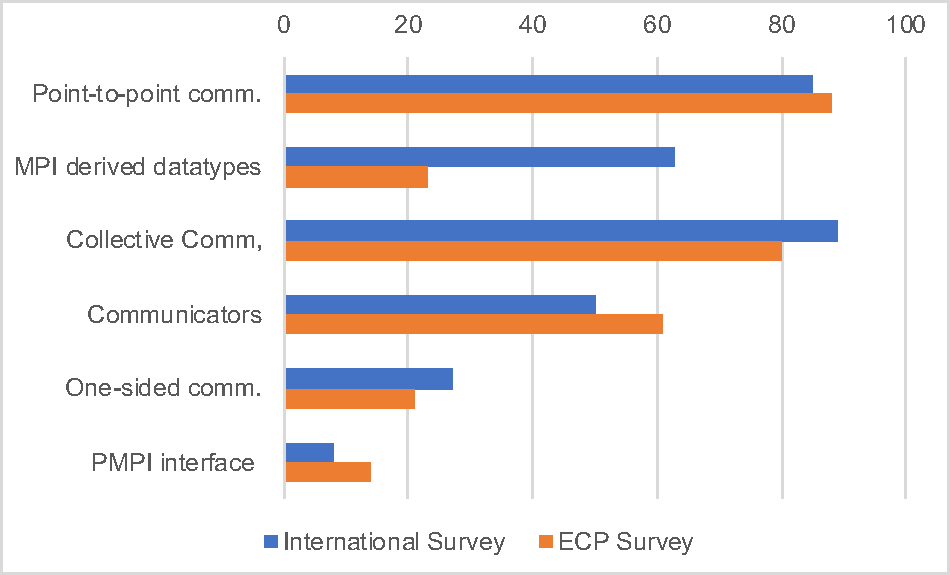
\includegraphics[width=0.8\hsize]{figs/ECP.pdf}
    \caption{Comparison of the result of asking using MPI aspects
      between ours and ECP}
    \label{fig:ecp-comparison}
  \end{center}
\end{figure}

There is a similar question of asking using MPI aspects in the ECP
survey. Figure~\ref{fig:ecp-comparison} compares the results of ours
and ECP survey on the common MPI aspects. Trends of both survey are
very similar excepting the usage of datatype. The percentage in our
survey is much higher than that of the ECP survey. 

\section{Summary and Future Work}

This large-scale international MPI survey reveals an uneven perception
of the MPI features, and a slow adoption of novel MPI
capabilities. Due to the page limit, only few of some of the most
interesting results of our survey are shown. We will publish more
results in the future.

%
\comment{
Based on the survey, our hypothesis is that due to the large impact of online
sources, new features have a slow propagation time from the MPI standard to
the first page of a Google search. If this unevenness is not addressed by the MPI
Forum itself, most new MPI features will continue to have a slow adoption, and
their usefulness will be limited to only niche communities.
}
% As the result of conducting an international, large-scale MPI survey,
% it is revealed that the uneven perception in the MPI features.
% Our hypothesis of this unevenness based on the survey results
% is that many MPI users nowadays learn MPI directly from online sources. If this
% unevenness will not be fixed then the new MPI features
% introduced by MPI Forum might also have a slow adoption by the user community.
% This can ruin the large effort of MPI Forum.

\section*{Acknowledgments}
We thank to those who participated in this survey and those who
helped us to distribute the questionnaire to their local
communities. We especially thank to MPI Forum members who gave us many
significant comments on the draft questionnaire.
This research is partially supported by the
NCSA-Inria-ANL-BSC-JSC-Riken-UTK Joint-Laboratory for Extreme Scale
Computing~\cite{JLESC}.

\bibliographystyle{acm}
\bibliography{../ref}

\end{document}
